\subsection*{Agents relay database errors in deployment and in a benchmark}

To test whether the problem arises outside a benchmark, we ran Biomni \citep{huang2026biomni}, an open-source biomedical agent, against the live UniProt and PubChem APIs and altered one field of selected responses in transit with an intercepting proxy (Methods). Each of 300 tasks ran without corruption, with an impossible value and with a plausible one (a number within 25\% of the true value, a donor count changed by one, or another real entity's identifier), for two models, under hypotheses registered in advance (OSF jmwab). The first run exposed the study's name to the agent through a directory path, and models can recognise evaluations from such cues \citep{needham2025evaluation}; we report a rerun in an isolated environment (Methods; Supplementary Note~1).

The corrupted value reached the agent in 559 and 583 of 600 corrupted runs (Fig.~\ref{fig:deploy}b). Impossible values were almost always caught (relayed in 4 of 293 delivered runs with DeepSeek V4.1 Flash and 4 of 283 with Gemini 3.8 Flash); plausible values were relayed in 17\% (50/290) and 21\% (57/276). Contrary to our registered prediction, fields with an exact derivation route were relayed more often, not less: protein length and mass in 36--62\% of plausible runs, organism and gene symbol in 0--8\% (odds ratios 17.2 and 6.9; Fig.~\ref{fig:deploy}c). Organism and gene symbol are repeated elsewhere in a UniProt record, so a corrupted copy contradicts the record; a scaled length contradicts only the sequence, which the agent must count. Gemini 3.8 Flash computed length or mass from the sequence in about half its runs and relayed half as often when it did (length 23\% against 50\%, mass 46\% against 79\%); DeepSeek never computed and relayed 37--52\%.

To separate detection from relay, we built a benchmark of 300 human proteins from UniProt \cite{uniprot2025} and 300 compounds from PubChem \cite{kim2025pubchem}, with lookup and threshold questions over ten templates, and ran ten models from five developers through a lookup tool (Methods). Clean accuracy was 98--100\% for every model. In corrupted runs one field of the target record held an impossible or a plausible value; plausible numeric corruptions scaled paired fields together, so the record stayed consistent, whereas impossible values changed one field and contradicted its partner. Asked, as in our registered prompt, to list anything that looked wrong, agents flagged impossible values in 75--100\% of runs yet relayed them in 32--93\% of protein and 38--91\% of chemistry runs, and relayed plausible values in 74--100\% and 93--100\% (Fig.~\ref{fig:bench}). The flags were specific: in impossible-value protein runs, 81\% cited a contradiction between fields of the record and 59\% the agent's memory of the protein (Methods). Without the request for concerns, agents still voiced doubt about most impossible values (36--84\% of runs, scored by a classifier validated against human labels at $\kappa = 0.84$) but rarely about plausible ones (0--29\%, against 43--97\% when asked), and relay rose in six of twelve cells, by up to 43 percentage points, and fell in one (Methods). Detection of plausible errors in the benchmark is therefore largely elicited by the prompt, and a plain prompt relays more.

\begin{figure}[t]
\centering
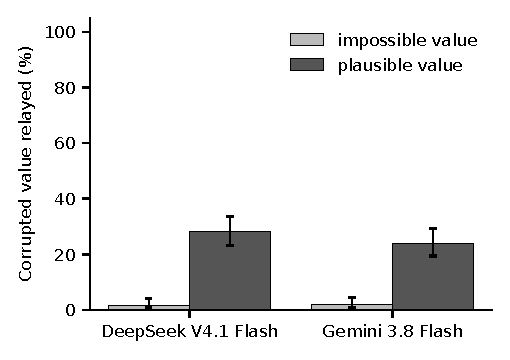
\includegraphics[width=\linewidth]{../figures/nmi_deployment.pdf}
\caption{\textbf{Study design and a deployed agent.} \textbf{a}, Corrupted values were injected between the database and the agent, in a tool layer or, for the deployed agent, an intercepting proxy; the agent's answer and concerns were scored. Bottom: the forms a corrupted record took (illustrative values). \textbf{b}, Biomni with live UniProt and PubChem APIs: share of corrupted runs in which the value was relayed, caught, or never requested (relayed/delivered at right). \textbf{c}, Relay of plausible values by field (shaded rows, compounds; filled circles, fields counted as having an exact derivation route (Methods); open diamonds, other fields), with 95\% Wilson intervals; numbers give relayed/delivered runs.}

\label{fig:deploy}
\end{figure}
\begin{figure}[t]
\centering
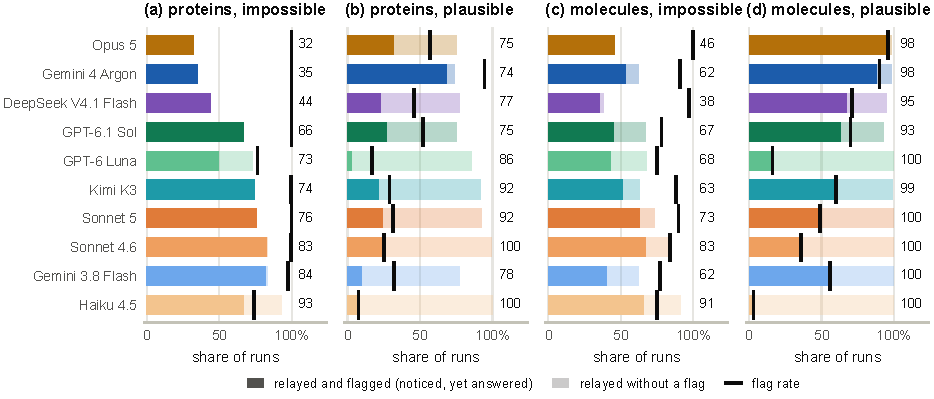
\includegraphics[width=\linewidth]{../figures/icml_main.pdf}
\caption{\textbf{Noticed yet answered.} Share of runs in which each model relayed the corrupted value into its final answer, for impossible and plausible values in the protein (\textbf{a}, \textbf{b}) and chemistry (\textbf{c}, \textbf{d}) benchmarks. Dark segments: relayed runs in which the agent also raised a concern; light segments: relayed without a concern; black ticks: share of all runs raising a concern. Runs used the registered prompt, which asks the agent to list concerns. Numbers give the relay rate (\%).}

\label{fig:bench}
\end{figure}
